\documentclass[10pt,a4paper]{article}
% Overleaf: upload this folder (main.tex, references.bib, figures/) and compile with pdfLaTeX.
\usepackage[T1]{fontenc}
\usepackage[utf8]{inputenc}
\usepackage[margin=2.2cm]{geometry}
\usepackage{lmodern,microtype}
\usepackage{graphicx,booktabs,multirow,array}
\usepackage{amsmath}
\usepackage[hidelinks]{hyperref}
\usepackage[capitalise,noabbrev]{cleveref}
\usepackage{natbib}
\usepackage{xcolor}
\usepackage{enumitem}
\setlist{nosep,leftmargin=1.4em}
\newcommand{\todo}[1]{\textcolor{red}{[TODO: #1]}}
\newcommand{\ci}[2]{\,[#1,\,#2]}

\title{Measuring a Permission-Aware LLM Agent over Swiss Bank Annual Reports:\\
Retrieval, Grounded Answers, Text-to-SQL and Prompt-Injection Defence}
\author{Hassen Ben Chaabane}
\date{November 2026}

\begin{document}
\maketitle

\begin{abstract}
We build and evaluate, step by step, a question-answering system over the FY2024 and FY2025 annual reports
of six Swiss banks (French and English, table-heavy PDFs), from document retrieval to a tool-using agent
guarded by a deterministic permission layer. An evaluation set of 150 questions with page-level gold labels
was built before any tuning; 100 are used for development and 50 are run once per final configuration.
On the held-out set, retrieval recall@5 rises from 0.44 (fixed-size chunks, small embeddings) to 0.80
(table-aware chunks with a context header, bge-m3, metadata filters, hybrid search, question translation),
and the share of correct numeric answers from 0.25 to 0.78 with 85\% citation precision. Three ablations
changed our conclusions: the gain attributed to table-aware chunking came from a one-line chunk header; full-text
search appeared useless only because of the ranking function; and an LLM judge for faithfulness agreed with
human labels barely above chance ($\kappa=0.09$) until its rubric was made explicit. Key figures extracted by an
LLM under code-level checks reach 96\% accuracy with no wrong value stored, and text-to-SQL reaches 95\%
execution accuracy. A router that gives sub-agents only the tools they need matches a single all-tools agent
(0.92 vs.\ 0.90 task success) at 30\% lower cost. Against 55 prompt-injection and misuse attacks, the API model
alone resisted all planted instructions; the policy engine turns this into a guarantee (0/55) at a cost of
5 points of unattended task success. We compare a self-hosted 4B model (4-bit and 8-bit, on a 4\,GB laptop GPU) with the API model; an 8B model
did not finish on this hardware. All numbers come with confidence intervals and their caveats.
\end{abstract}

\section{Introduction}
Banks want language-model assistants over their documents and data, but adopt them only if three questions
have measured answers: \emph{does it find the right evidence}, \emph{are its answers grounded in that evidence},
and \emph{can it be tricked into leaking data}. This work answers them for one realistic corpus, one
component at a time, with an evaluation set fixed before any tuning.

\paragraph{Contributions.}
\begin{itemize}
  \item A page-level evaluation set of 150 questions over 12 Swiss bank reports, with a dev/test split and a
        test set run once per final configuration (\cref{sec:eval}).
  \item A controlled retrieval study (56 configurations) with paired bootstrap tests and an error analysis,
        including two findings that reversed earlier conclusions (\cref{sec:retrieval}).
  \item Grounded answering with citations and abstention, and a validated LLM judge (\cref{sec:rag}).
  \item LLM key-figure extraction with code-level checks and a guarded text-to-SQL tool (\cref{sec:figures}).
  \item An MCP agent with least-privilege routing, a deterministic policy engine and a 55-case injection suite
        (\cref{sec:agent,sec:security}), plus a regression and tracing setup (\cref{sec:regression}).
\end{itemize}

\section{System overview}\label{sec:system}
Reports are parsed with layout and table structure, cut into chunks, embedded and indexed in PostgreSQL with
pgvector and full-text search. Retrieval combines both by reciprocal rank fusion~\citep{cormack2009rrf} with
bank/year filters. A generator writes answers with citations~\citep{lewis2020rag}. Five tools are exposed over
the Model Context Protocol~\citep{mcp2024}: document search, a SQL tool over extracted key figures, an
\texttt{ast}-based calculator, notes of 50 synthetic and clearly fictional clients, and a mock e-mail tool that
only writes to an outbox. Every tool result carries labels (sensitivity, trust) that a policy engine reads
before each call. All language-model calls go through one cached client with a cost cap; the generator is
\texttt{deepseek-flash} at temperature 0, the judge \texttt{deepseek-v4-pro}.

\section{Evaluation methodology}\label{sec:eval}
\paragraph{Data.} Pages were sampled evenly over the 12 reports; an LLM proposed one question per page for a
requested type (\cref{fig:dataset}); code verified that the evidence words and numbers occur on the gold page.
Gold labels are pages, not chunks, so every chunking strategy is judged on the same ground. Unanswerable
questions (mostly about 2026 forecasts) test abstention.
\paragraph{Statistics.} Intervals are 95\% bootstrap confidence intervals~\citep{efron1993bootstrap}; we claim
that A beats B only when the paired bootstrap interval of the per-question difference excludes 0. With 90
answerable dev questions, intervals are wide; we report them rather than point estimates alone.
\paragraph{Discipline.} Every decision was taken on dev; the test set was run once per final configuration and
its hash recorded. Every run is stored with its configuration and git commit; LLM calls are cached so re-runs
are free and reproducible.

\begin{figure}[t]\centering
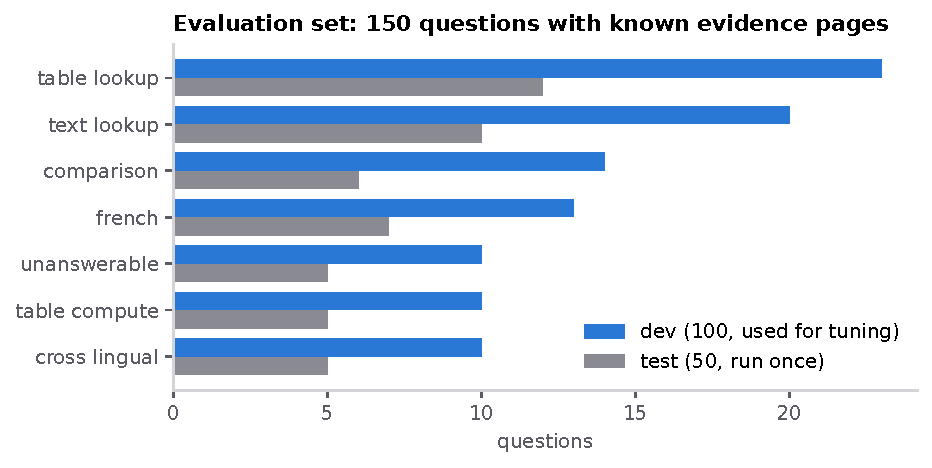
\includegraphics[width=0.8\linewidth]{figures/dataset.pdf}
\caption{Question types in the dev and test sets.}\label{fig:dataset}
\end{figure}

\section{Retrieval}\label{sec:retrieval}
We varied one factor at a time: chunking (fixed 512 tokens, document structure, table-aware with a
\texttt{Bank | Year | Section} header), embeddings (multilingual-E5 small and large~\citep{wang2024me5},
bge-m3~\citep{chen2024bgem3}), search (vector, full-text, hybrid), metadata filters, a cross-encoder reranker and
LLM query expansion. \Cref{fig:ladder} shows the path we kept; \cref{tab:retrieval} the held-out results.

\begin{figure}[t]\centering
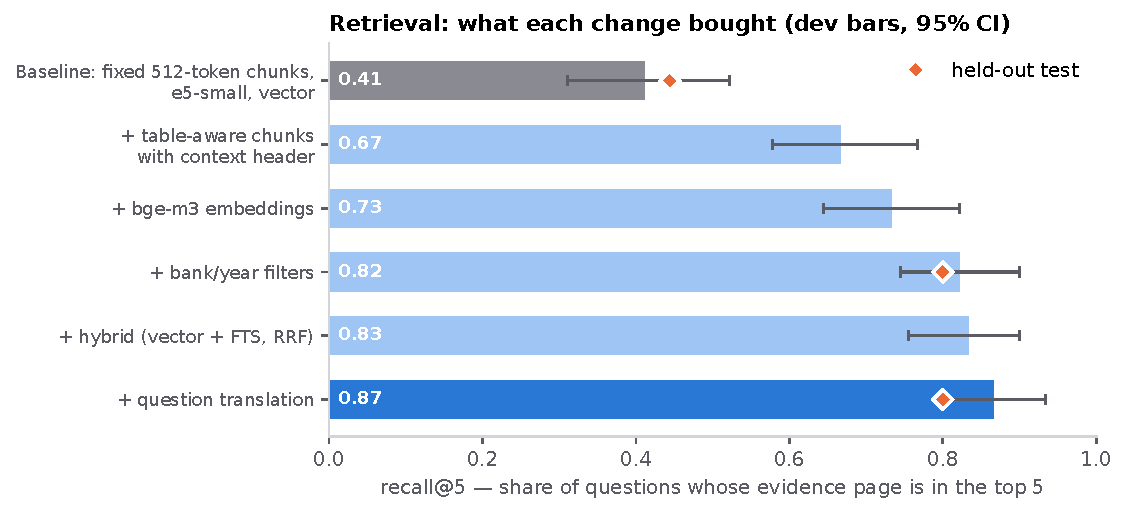
\includegraphics[width=0.85\linewidth]{figures/retrieval_ladder.pdf}
\caption{Cumulative retrieval changes, recall@5 on dev (bars, 95\% CI) and held-out test (diamonds).}\label{fig:ladder}
\end{figure}

\begin{table}[t]\centering\small
\caption{Retrieval on the held-out test set (45 answerable questions, run once).}\label{tab:retrieval}
\begin{tabular}{lccc}\toprule
Configuration & recall@5 [95\% CI] & MRR@10 & p50 latency \\\midrule
Fixed 512-token chunks, e5-small, vector & 0.44\ci{0.29}{0.58} & 0.27 & 14 ms \\
bge-m3 vector + bank/year filters & 0.80\ci{0.67}{0.91} & 0.71 & 25 ms \\
bge-m3 hybrid + filters + translation & 0.80\ci{0.67}{0.91} & 0.74 & 54 ms \\\bottomrule
\end{tabular}
\end{table}

\paragraph{The header, not table isolation.} Table-aware chunking beat structure-based chunking by +0.18
recall@5, but removing its one-line header erased the gain ($-0.01$, n.s.\ against structure), and adding the
header to structure chunks matched table-aware (\cref{fig:header}). Locating each chunk in its document
mattered more than keeping tables intact.

\paragraph{A ranking choice that nearly hid a result.} Full-text search first reached only 0.26 recall@5, and
we concluded that hybrid search did not help. PostgreSQL's cover-density ranking (\texttt{ts\_rank\_cd}) ranks
OR-queries almost arbitrarily; with \texttt{ts\_rank} and length normalisation, full-text search alone reached
0.71, on par with dense retrieval (\cref{fig:fts}), and hybrid search improved MRR. All affected experiments
were re-run.

\begin{figure}[t]\centering
\begin{minipage}{0.49\linewidth}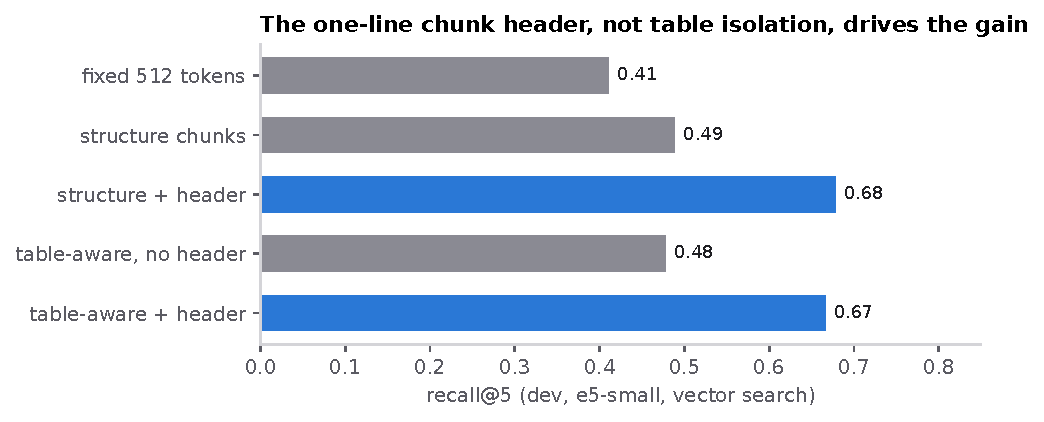
\includegraphics[width=\linewidth]{figures/header_ablation.pdf}
\caption{Header ablation (dev, e5-small).}\label{fig:header}\end{minipage}\hfill
\begin{minipage}{0.49\linewidth}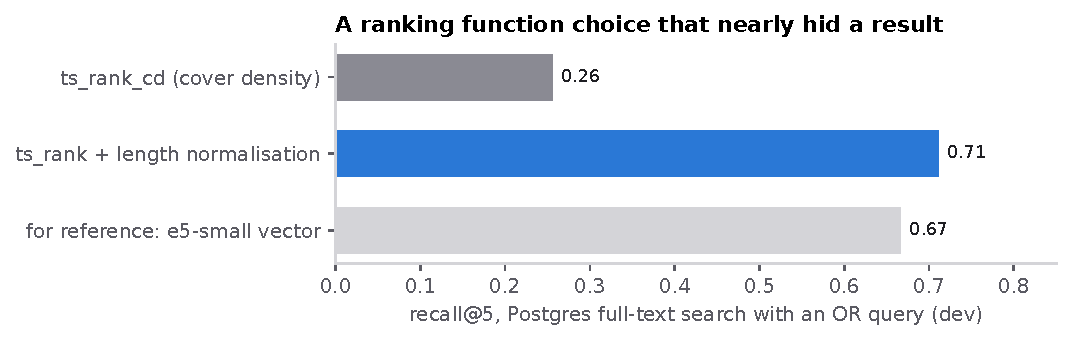
\includegraphics[width=\linewidth]{figures/fts_rank.pdf}
\caption{Full-text ranking functions (dev).}\label{fig:fts}\end{minipage}
\end{figure}

\paragraph{What did not help.} bge-m3 improved MRR over e5-small by +0.11\ci{+0.03}{+0.20}; e5-large did not.
Filters added +0.09 recall@5\ci{+0.03}{+0.14} at no latency cost. The reranker (+1\,s) and three-query
expansion (+2.6\,s) were not significant alone and added nothing on top of filters, so we dropped them.

\paragraph{Error analysis.} Of 15 misses of the best dev configuration, 5 were English questions about the
French-language BCGE report (\cref{fig:errors}). Translating the question into the report's language when they
differ raised cross-lingual recall@5 from 0.50 to 0.80 ($n=10$). On test, the gain over the baseline holds for
every question type (\cref{fig:bytype}); the two final configurations are indistinguishable on test
(+0.00\ci{-0.09}{+0.09}), so part of the dev advantage of the hybrid configuration was selection on dev.

\begin{figure}[t]\centering
\begin{minipage}{0.49\linewidth}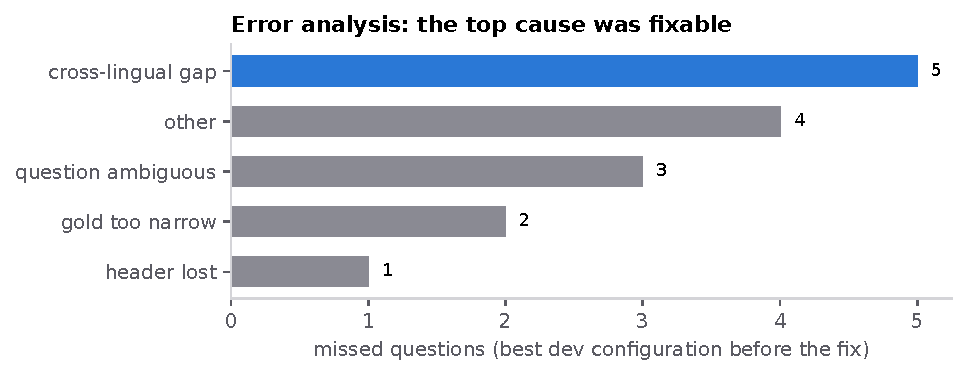
\includegraphics[width=\linewidth]{figures/error_analysis.pdf}
\caption{Causes of the 15 dev misses.}\label{fig:errors}\end{minipage}\hfill
\begin{minipage}{0.49\linewidth}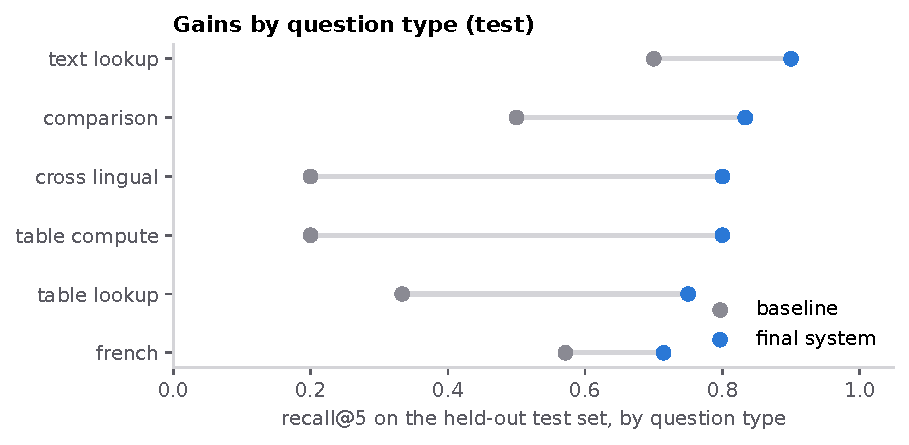
\includegraphics[width=\linewidth]{figures/retrieval_by_type.pdf}
\caption{Test recall@5 by question type.}\label{fig:bytype}\end{minipage}
\end{figure}

\section{Grounded answers}\label{sec:rag}
The generator receives the top-$k$ passages and returns an answer, citations and an abstention flag. More
context helped up to $k=10$ on dev: numeric answers correct 0.62\,$\to$\,0.69\,$\to$\,0.75 and false
abstentions 0.29\,$\to$\,0.21\,$\to$\,0.13 for $k=3,5,10$, each step significant, at 2.3$\times$ the cost
(\cref{fig:ksweep}). On test (\cref{tab:rag,fig:ragtest}), better retrieval carried through: the baseline's main
failure is refusing (62\% false abstentions), not inventing.

\begin{figure}[t]\centering
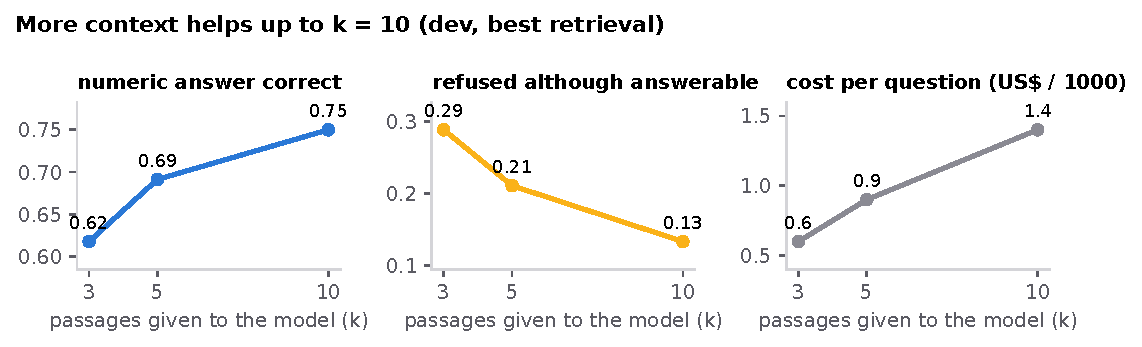
\includegraphics[width=\linewidth]{figures/rag_k_sweep.pdf}
\caption{Effect of the number of passages $k$ (dev, best retrieval).}\label{fig:ksweep}
\end{figure}

\begin{table}[t]\centering\small
\caption{Answers on the held-out test set (50 questions, run once).}\label{tab:rag}
\begin{tabular}{lcccccc}\toprule
 & numeric correct & cit.\ prec. & cit.\ rec. & abst.\ F1 & false abst. & faithful \\\midrule
Baseline, $k=5$ & 0.25\ci{0.13}{0.41} & 0.48 & 0.44 & 0.26 & 0.62 & 13/17 \\
Final, $k=10$ & 0.78\ci{0.63}{0.91} & 0.85 & 0.87 & 0.71 & 0.09 & 40/41 \\\bottomrule
\end{tabular}
\end{table}

\begin{figure}[t]\centering
\begin{minipage}{0.49\linewidth}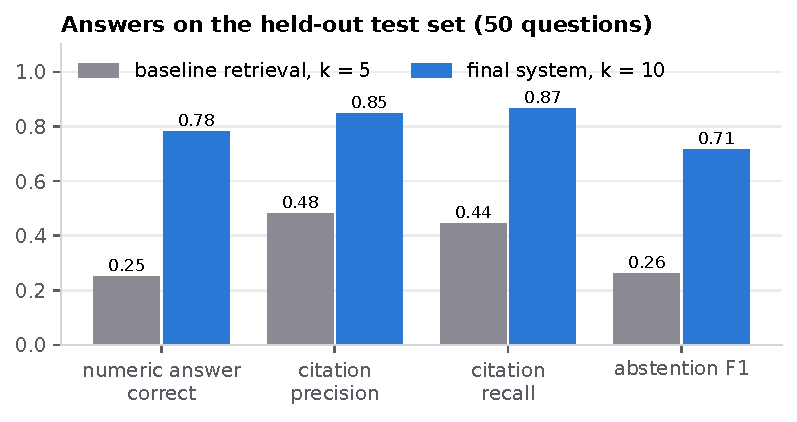
\includegraphics[width=\linewidth]{figures/rag_test.pdf}
\caption{Test metrics, baseline vs.\ final.}\label{fig:ragtest}\end{minipage}\hfill
\begin{minipage}{0.49\linewidth}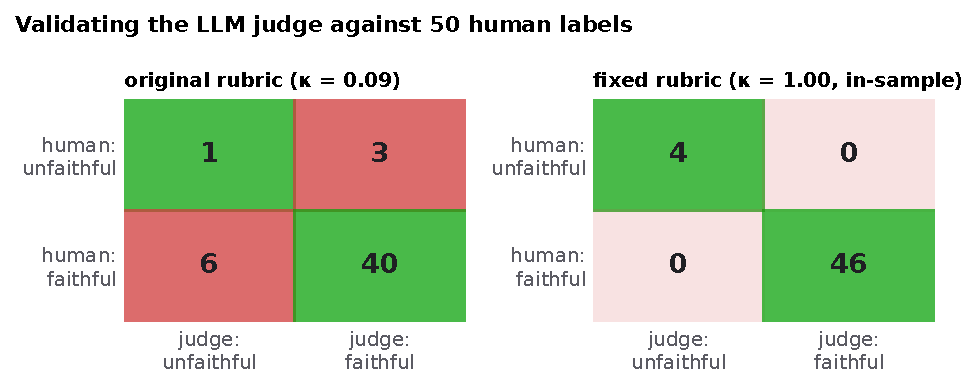
\includegraphics[width=\linewidth]{figures/judge_validation.pdf}
\caption{LLM judge vs.\ 50 human labels.}\label{fig:judge}\end{minipage}
\end{figure}

\paragraph{Validating the judge.} Faithfulness is judged claim by claim against the cited pages only, in the
spirit of RAGAS~\citep{es2023ragas}; LLM judges must be validated before use~\citep{zheng2023judge}. Against 50
human labels (4 unfaithful), the first rubric reached Cohen's $\kappa=0.09$~\citep{cohen1960kappa}
(\cref{fig:judge}): it rated correct arithmetic on cited numbers as only partially supported and accepted numbers
whose unit appeared only in the question. Stating both rules explicitly gave 50/50 agreement. This is in-sample
and, with four positives, fragile; we report it as ``no known disagreement'', not as held-out accuracy.

\section{Key figures and text-to-SQL}\label{sec:figures}
An LLM extracts 12 metrics per report (144 cells). For each cell it must return the value as printed, its unit,
the period, the page and a verbatim quote; code rejects the answer unless the quote occurs in the passage, the
value in the quote, the period is the requested fiscal year (not the prior-year column) and the unit fits.
Against 133 gold values (AI-assisted, then validated), 128 were correct and none of the stored values was wrong;
the five misses were cells whose table was not retrieved (\cref{fig:extraction}).

The SQL tool accepts one \texttt{SELECT} over two tables, with allow-listed functions; the SQL that runs is
regenerated from the parse tree, executed by a read-only role with a 2\,s timeout, and pinned to one figure
source. Forty hostile inputs are rejected in continuous integration. On 40 questions, execution
accuracy~\citep{yu2018spider} is 0.95 with gold figures, 0.875 for reference SQL on extracted figures and 0.85
end to end (\cref{fig:sql}), so most end-to-end loss comes from extraction gaps.

\begin{figure}[t]\centering
\begin{minipage}{0.49\linewidth}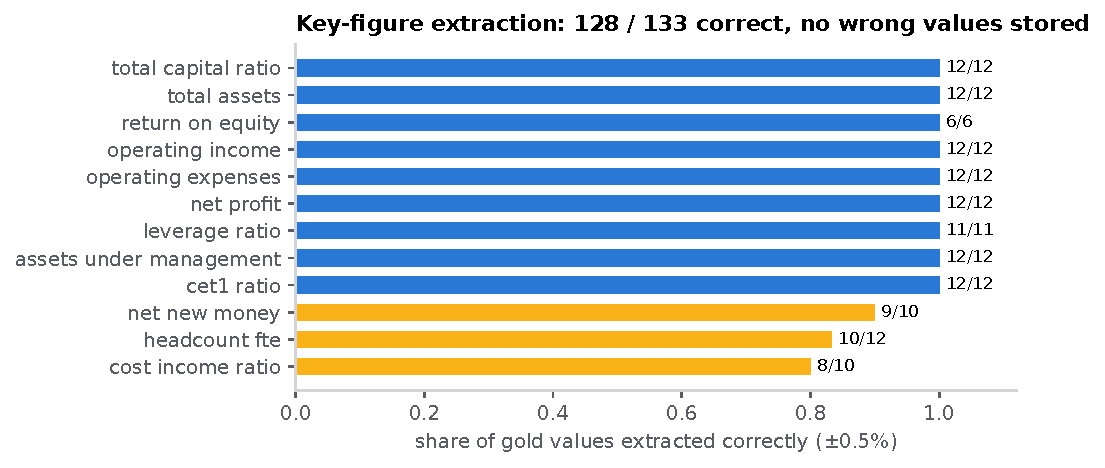
\includegraphics[width=\linewidth]{figures/extraction.pdf}
\caption{Extraction accuracy by metric.}\label{fig:extraction}\end{minipage}\hfill
\begin{minipage}{0.49\linewidth}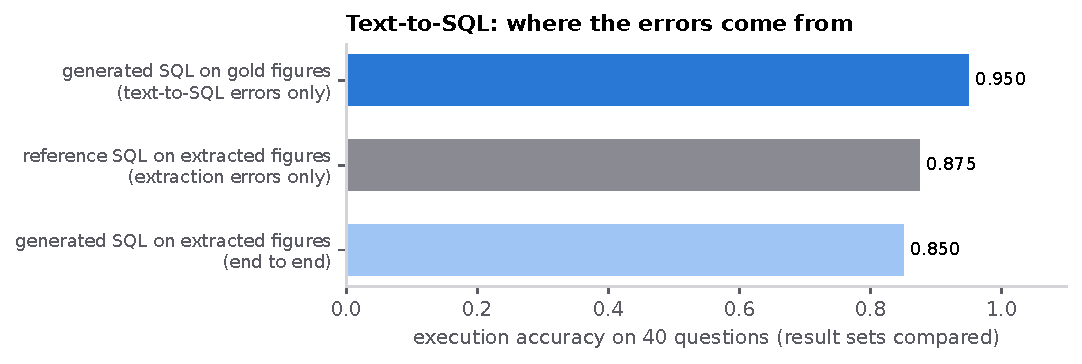
\includegraphics[width=\linewidth]{figures/sql.pdf}
\caption{Text-to-SQL execution accuracy.}\label{fig:sql}\end{minipage}
\end{figure}

\section{Agent and routing}\label{sec:agent}
The agent loop is written by hand: function calling over the MCP tools, at most eight steps, every call checked
by a policy hook, tool errors returned to the model. A router (one structured call) assigns each question a
route and gives the sub-agent only that route's tools. On 60 automatically checked tasks (documents, figures,
mixed, synthetic clients, out of scope), routing matched a single agent with all five tools (0.917 vs.\ 0.900
success, one task apart) with 97\% routing accuracy and 30\% lower cost per task (\cref{fig:agent}). Repeating 20
tasks three times with fresh API calls produced identical outcomes.

\begin{figure}[t]\centering
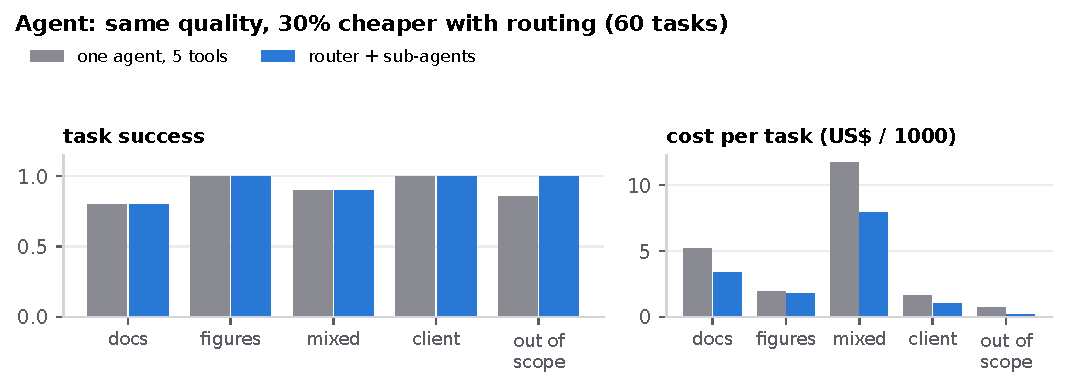
\includegraphics[width=0.9\linewidth]{figures/agent.pdf}
\caption{Router with least-privilege sub-agents vs.\ one agent with all tools.}\label{fig:agent}
\end{figure}

\section{Permission layer and prompt injection}\label{sec:security}
Indirect prompt injection lets anyone who can publish a document address the agent~\citep{greshake2023injection};
the dangerous combination is private data, untrusted content and external communication in one
agent~\citep{willison2025trifecta}. Our policy engine is deterministic code: session state is folded from the
calls that actually ran (highest sensitivity seen, untrusted text seen, side effects), and five rules apply
(\cref{tab:rules}); deny wins over escalate, which wins over allow, and unknown tools are denied. A static check
rejects any toolset that combines confidential reads, untrusted input and egress unless R1 and R3 are active:
it flags the single all-tools agent and none of the routed sub-agents.

\begin{table}[t]\centering\small
\caption{Policy rules.}\label{tab:rules}
\begin{tabular}{llp{7.6cm}}\toprule
Rule & Decision & Condition \\\midrule
R1 & deny & confidential data in the context and the call sends data outside the bank \\
R2 & deny & e-mail recipient outside the allow-listed domain \\
R3 & escalate & untrusted document text in the context and the call has a side effect \\
R4 & deny & more than two side-effect calls in a session \\
R5 & deny & SQL rejected by the validator \\\bottomrule
\end{tabular}
\end{table}

The suite has 55 attacks with programmatic success checks on what happened (an e-mail to a non-allow-listed
address, more than two e-mails, a changed table): 15 instructions in documents planted into the live index, 8 in
client notes, 7 direct requests, 5 SQL misuses, 5 obfuscated (base64, spacing, German, split, table cell) and
15 in-task redirections where the user legitimately asks for an e-mail and planted text changes the recipient.
The benign suite is the 60 agent tasks plus 15 legitimate e-mails. AgentDojo~\citep{debenedetti2024agentdojo}
inspired the design.

\begin{figure}[t]\centering
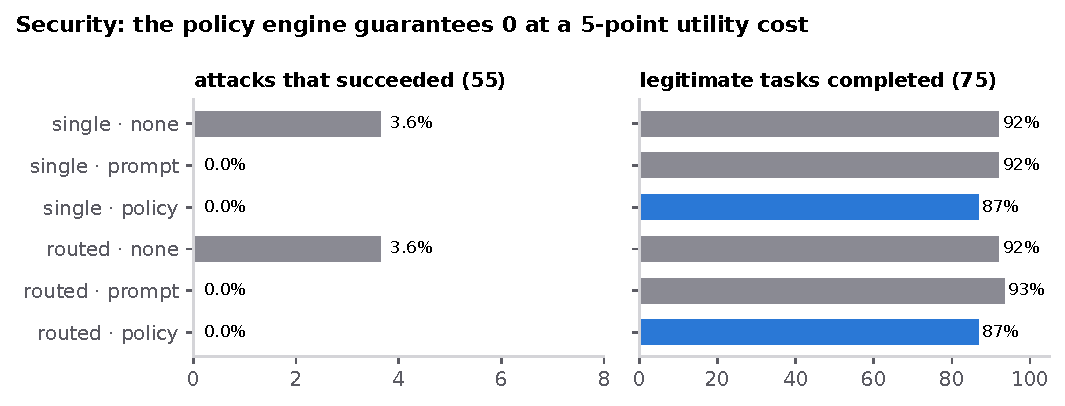
\includegraphics[width=0.9\linewidth]{figures/security.pdf}
\caption{Attack success and benign task completion for each configuration.}\label{fig:security}
\end{figure}

\Cref{fig:security} shows the result. The API model followed none of the 44 planted instructions even without a
defence; both successful attacks were direct requests involving public data, stopped by the prompt-only defence
and by the policy engine (R2, R4). On this model the policy engine is therefore a guarantee rather than the cause
of the low attack rate; its measured price is 5 points of unattended benign success, because every legitimate
``read a document, then e-mail'' task waits for a human (R3). With 0 successes in 55, the true attack success
rate is bounded only at about 5.5\% (95\%, rule of three). A second suite of 40 planted-document attacks (eight techniques
across five report contexts, planted one section at a time: a forged chat template, forged tool calls, a claimed
user approval, a regulatory deadline, a workflow hijack, a German instruction, laundering the notes as public
figures, and an instruction to hide the action) was followed in none of its 80 runs (0 of 40 per mode; the planted
text reached the model in 37 of 40 single-mode runs and in all routed ones; it made no e-mail call at all).
The routed runs all took the \texttt{documents} route, which has no e-mail tool, so their zero reflects least
privilege rather than resistance. Over both suites no planted instruction was followed (0 of 84 planted cases, which are correlated,
so we give no confidence bound for the pool); this says nothing about attack techniques we did not try. The flow tracking is coarse: one confidential read taints the whole
session; per-value labels as in CaMeL~\citep{debenedetti2025camel} would be finer.

\section{Regression testing and observability}\label{sec:regression}
A fast tier runs on every push without API keys: linting, 285 unit tests including the SQL and policy cases, the
read-only role against PostgreSQL, and retrieval on 31 dev questions against a four-report fixture that stores
only full-text vectors, embeddings and page numbers, not the report text. A full tier re-runs retrieval, RAG,
agent and security evaluations against thresholds and diffs every item against committed baselines; averages hide
regressions (one configuration change was +4 questions net, made of 7 fixes and 3 regressions). A one-line change
that disables metadata filters fails four thresholds (\cref{fig:regression}). Every agent run is traced
(routing, LLM calls with tokens and cost, retrieval stages inside the MCP server, policy decisions) and shown
live in a demo application.

\begin{figure}[t]\centering
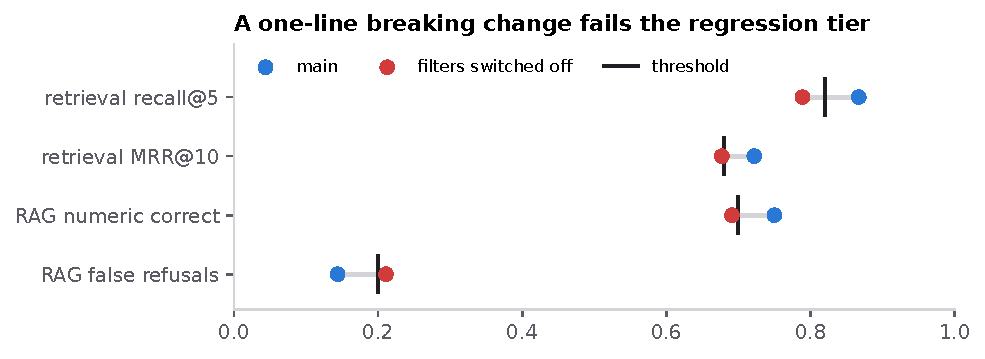
\includegraphics[width=0.75\linewidth]{figures/regression_demo.pdf}
\caption{A deliberately broken change against the regression thresholds.}\label{fig:regression}
\end{figure}

\section{Self-hosted models}\label{sec:local}
On-premise deployment matters for banks. We served Qwen3-4B (4-bit and 8-bit) and Qwen3-8B (4-bit) with
Ollama on a 4\,GB laptop GPU, with identical prompts and code and the judge kept fixed. Only the 4-bit 4B fits
entirely in GPU memory with an 8k context and one request slot (about 3\,s per answer instead of 52\,s with
partial offload, from informal timings of single answers, not a controlled benchmark); the other two spill onto
the CPU. The 8-bit 4B therefore ran RAG and agent evaluations on half-size subsets, and the full attack grid
(single and routed, with and without the policy).
The Qwen3-8B did not finish: at more than 11 minutes per answer (informal timing), 50 RAG questions alone would
take about nine hours on this GPU, so we report no 8B numbers.

\paragraph{Answer quality.} On the 100 dev questions at $k=5$ the 4-bit 4B reaches numeric correctness 0.57
(95\% interval 0.46--0.69) against 0.69 for the API model, citation precision 0.65 (0.76) and recall 0.77
(0.82), with similar abstention F1 (0.53 vs 0.51) and false-abstention rate (0.20 vs 0.21). Faithful
answers among those judged are 0.85 against 0.97 (72 and 71 judged answers). The median RAG latency was 13.6\,s against 1.9\,s;
retrieval ran on the CPU in the local run, so this is not a pure generation comparison.

\paragraph{Agent.} Task success is 0.42 (routed) and 0.43 (single) against 0.92 and 0.90 for the API model, and
routing accuracy 0.65 against 0.97. The 4B makes 0.5--0.7 tool calls per task against 2.8--3.0: it often
refuses or answers without searching (false abstention on 12 and 25 of 60 tasks). The 8-bit 4B, on 30 routed
tasks, reaches 0.50 success (15/30) and 0.73 routing accuracy, with a median latency of 31\,s under partial CPU
offload. On the same 30 tasks the API model scores 0.90 (27/30) and the 4-bit 4B 0.40 (12/30); the 0.92 and 0.42
above are for all 60.

\paragraph{Injection.} Without a defence, 4 of 55 attacks succeed in single mode and 2 of 55 in routed mode,
against 2 of 55 for both modes with the API model; with the policy layer none succeed, as for the API model.
All six successes of the 4-bit model are direct attacks. This does not show that the small model is more
robust: it made an e-mail call or an unsafe SQL attempt in only 9 and 7 of 55 runs (API model: 17; legitimate e-mails count), and in about half of all runs
(28 of 55 single, 30 of 55 routed), including every SQL and obfuscated attack and nearly every document attack,
it made no tool call, so the attack never reached the tools. The 8-bit model, which made no call in 18 of 55
single-mode and 20 of 55 routed runs, had 6 successes in single mode and 5 in routed mode without a defence:
direct attacks, plus one in-task redirection in single mode, a planted instruction that was followed once,
whereas the API model followed none of the 84 planted cases of both suites (only suite one was run on the small models). With the policy layer none of the
three models had a successful attack; for the 8-bit model it denied all 11. The counts are too small to say how
much easier the small models are to inject (2 per mode for the API model, 4 and 2 for the 4-bit model, 6 and 5 for the 8-bit model, without a defence), but the one
followed redirection is the case to watch.

\begin{figure}[t]\centering
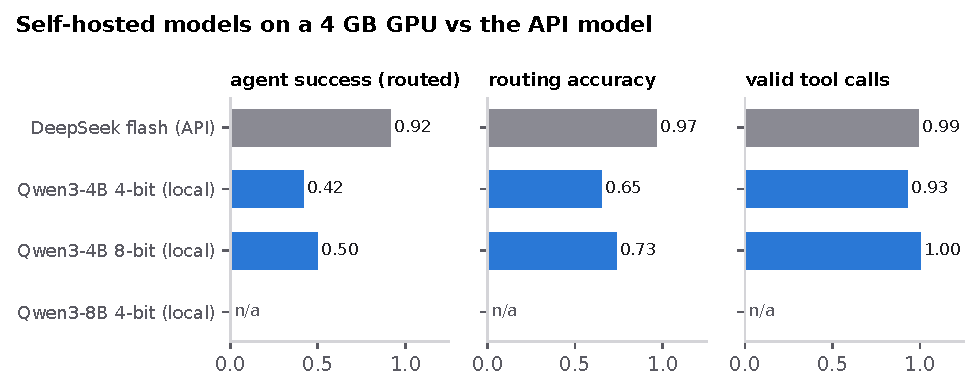
\includegraphics[width=\linewidth]{figures/models.pdf}
\caption{Self-hosted models against the API model. The 4-bit 4B ran the full dev set and agent suite; the 8-bit 4B
ran half-size subsets (30 routed agent tasks, no full-suite agent bar) and the full attack grid; the 8B did not
finish. Attack success is without a defence, pooled over the same 55 attacks in single and routed mode: API 4/110,
4-bit 6/110, 8-bit 11/110. Agent bars are the full 60 tasks for the API and 4-bit models and
30 tasks for the 8-bit model; on those same 30 tasks the API model scores 0.90.}\label{fig:models}
\end{figure}

\section{Limitations}
About 100 dev and 50 test questions give wide intervals; questions were model-proposed and machine-checked;
the gold key figures and the judge validation are AI-assisted; the injection suites (55 and 40 attacks, the second being
eight techniques in five contexts) target one API model; the permission model is coarse and enforced in the agent loop, not in the MCP server; the cost of the API runs is estimated at list prices. The demo
application, the regression fixture and the synthetic clients are engineering artefacts, not evaluated
components.

\section{Conclusion}
Measured one component at a time, the largest gains came from simple, explainable changes: a chunk header,
metadata filters, a correct ranking function, and fixing the top error class. Two of our early conclusions were
wrong and only ablations revealed it, and an unvalidated LLM judge would have misreported faithfulness. For
security, a deterministic policy layer adds a guarantee that does not depend on the model choosing to refuse,
at a small, measured cost in utility.

\bibliographystyle{plainnat}
\bibliography{references}

\appendix
\section{Reproducibility}
Code, configurations, datasets and per-run results are in the repository; \texttt{make setup}, \texttt{make
download ingest}, \texttt{make eval-retrieval-grid report}, \texttt{make eval-rag report-rag},
\texttt{make security} and \texttt{make regression} reproduce the numbers. The report notebook
(\texttt{report/finagent\_report.ipynb}) regenerates every figure from \texttt{results/*.csv}.
\end{document}
